%%%%%%%%%%%%%%%%%%%%%%%%%%%%%%
%  This Beamer template was created by Cameron Bracken.
%  Anyone can freely use or modify it for any purpose
%  without attribution.
%
%  Last Modified: January 9, 2009
%

\documentclass[xcolor=x11names,compress]{beamer}

% General document %%%%%%%%%%%%%%%%%
\usepackage{graphicx}
\usepackage{tikz}
\usepackage[brazilian]{babel}
\usepackage[utf8]{inputenc}
\usepackage[T1]{fontenc}
\usepackage{mathtools}
\usepackage{amsfonts}
\usepackage{graphicx}
\usepackage{booktabs}
\usepackage{url}
\usetikzlibrary{decorations.fractals}
%%%%%%%%%%%%%%%%%%%%%%%%%%%

% Beamer Layout %%%%%%%%%%%%%%%%%
\useoutertheme[subsection=false,shadow]{miniframes}
\useinnertheme{default}
\usefonttheme{serif}
\usepackage{palatino}

\setbeamerfont{title like}{shape=\scshape}
\setbeamerfont{frametitle}{shape=\scshape}

\definecolor{azulzinho}{RGB}{248,249,254}
\setbeamercolor*{background canvas}{bg=azulzinho}
\setbeamercolor*{lower separation line head}{bg=DeepSkyBlue4} 
\setbeamercolor*{normal text}{fg=black,bg=white} 
\setbeamercolor*{alerted text}{fg=red} 
\setbeamercolor*{example text}{fg=black} 
\setbeamercolor*{structure}{fg=black} 
 
\setbeamercolor*{palette tertiary}{fg=black,bg=black!10} 
\setbeamercolor*{palette quaternary}{fg=black,bg=black!10} 

\renewcommand{\(}{\begin{columns}}
\renewcommand{\)}{\end{columns}}
\newcommand{\<}[1]{\begin{column}{#1}}
\renewcommand{\>}{\end{column}}
%%%%%%%%%%%%%%%%%%%%%%%%%




\begin{document}


%%%%%%%%%%%%%%%%%%%%%%%%%%%
%%%%%%%%%%%%%%%%%%%%%%%%%%%
\section{\scshape Introdução}
\begin{frame}
\title{\LARGE Associação de Molas}
\author{
	Lucas Magno, Fernando Augusto Joaquim e Maurício Branbilla\\[0.2cm]
	{\it \footnotesize Física Experimental II 	\\Professor Alexandre Suaide}\\[0.3cm]
	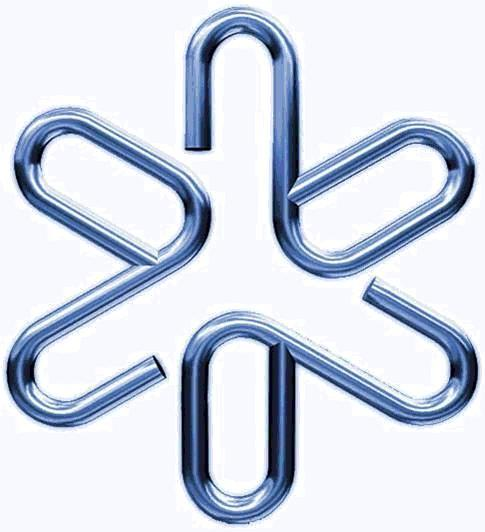
\includegraphics[scale=0.2]{logo_if_azul}\\[0.5cm]
	\today	
}
\titlepage
\end{frame}

%%%%%%%%%%%%%%%%%%%%%%%%%%%
%%%%%%%%%%%%%%%%%%%%%%%%%%%

\subsection{Objetivos}

\begin{frame}{Objetivos}
	\begin{itemize}
		\item Observar a constante elástica resultante de sistemas de molas
		\item Comparar com previsões teóricas a partir das constantes individuais
		\item Verificar o intervalo de validade do modelo teórico
	\end{itemize}
\end{frame}



\subsection{Modelos teóricos}

\begin{frame}{Modelos teóricos}
	\begin{itemize}
		\item Molas em paralelo
			\[ K_{R} = K_{1}+K_{2}\]
		\item Molas em série
			\[ \frac{1}{K_{R}} = \frac{1}{K_{1}} + \frac{1}{K_{2}} \]
		\item Gráfico
			\[M = \frac{K_{R}}{g}X\]
	\end{itemize}
\end{frame}

%%%%%%%%%%%%%%%%%%%%%%%%%%%
%%%%%%%%%%%%%%%%%%%%%%%%%%%

\section{\scshape Métodos}


\subsection{Aparato Experimental}

\begin{frame}{Aparato Experimental}
	\begin{itemize}
		\item Molas
		\item Pesos
		\item Suporte vertical para as molas
		\item Réguas
		\item Máquina fotográfica
	\end{itemize}
\end{frame}



\subsection{Procedimento}

\begin{frame}{Procedimento}
	\begin{itemize}
		\item Método estático
		\item Diferentes combinações de molas
		\item Variação dos pesos
		\item Registro fotográfico das posições
		\item Criação de gráficos e análise destes
	\end{itemize}
\end{frame}

%%%%%%%%%%%%%%%%%%%%%%%%%%%
%%%%%%%%%%%%%%%%%%%%%%%%%%%

\section{\scshape Análise}


\subsection{Primeiro Ajuste}

\begin{frame}{Primeiro Ajuste}
	\begin{itemize}
		\item Gráfico\\
			\includegraphics{M1+3.png}
	\end{itemize}
\end{frame}


\begin{frame}{Primeiro Ajuste}
	\begin{itemize}
		\item Previsão teórica: \[K_{R} = 13.21 \pm 0.14 \quad N/m\] 
		\item Obtido: \[K_{R} = 12.31 \pm 0.18 \quad N/m\]\\
			\[Z = 3.99\]\\
			\[\frac{\chi^{2}}{NDF} = 6.14\]
	\end{itemize}
\end{frame}



\subsection{Segundo Ajuste}

\begin{frame}{Segundo Ajuste}
	\begin{itemize}
		\item Gráfico\\
			\includegraphics{M1+3Linear.png}
	\end{itemize}
\end{frame}


\begin{frame}{Segundo Ajuste}
	\begin{itemize}
		\item Previsão teórica: \[K_{R} = 11.56 \pm 0.35 \quad N/m\] 
		\item Obtido: \[K_{R} = 11.22 \pm 0.32 \quad N/m\]\\
			\[Z = 0.72\]\\
			\[\frac{\chi^{2}}{NDF} = 0.58\]
	\end{itemize}
\end{frame}

%%%%%%%%%%%%%%%%%%%%%%%%%%%
%%%%%%%%%%%%%%%%%%%%%%%%%%%

\section{\scshape Conclusão}


\subsection{Conclusão}

\begin{frame}{Conclusão}
	\begin{itemize}
		\item Massa mínima para comportamento linear
		\item Massa máxima a fim de evitar deformação
		\item Excelente compatibilidade entre o sistema e o modelo teórico no intervalo apropriado
	\end{itemize}
\end{frame}

\end{document}
